%#! platex 000main.tex
\chapter{結果}
  \label{chap:result}
  表6.1はアンケート結果である. ほとんどの場合でラスタスキャンのほうが人に近いという結果がでた. 
  \begin{table}[h]
  \caption{アンケート結果\label{アンケート結果}}
  \label{tab:sample-tab}
  \begin{center}
      \vskip 1zh
      \small
      \begin{tabular}{c|c|c} \hline
        画像         & ラスタスキャン(人)   & 端点(人)  \\ \hline
       	1            & 6  				& 3   \\ 
        2            & 6	  			& 3   \\ 
        3            & 7   				& 2   \\ 
        4            & 6   				& 3   \\ 
        5            & 5   				& 4   \\ 
        6            & 5   				& 4   \\ 
        7            & 6   				& 3   \\ 
        8            & 2   				& 7   \\ 
        9            & 7   				& 2   \\ 
        10           & 6   				& 3   \\ \hline
      \end{tabular}
  \end{center}
\end{table}
  \section{考察}
  \label{sec:consideration}
  端点は線を辿るようにしたので,逆に一筆書きのようになり,不自然な書き方になったと考えられる. 実際に7枚の画像が目や鼻,耳などから頭上へ繋がって下から上へと描かれた.
  また,最も近い端点に移動すれば,近似的に線を描けると仮定したが,交点を考慮する必要があった. そのため,本来とは違う軌道になることが多くなったと考えられる. 
  エッジとノイズはトレードオフ関係にある(文献\cite{4})ため,エッジを用いるなら,途切れた線を補間する必要があると考えられる.
  \section{描画の結果}
  \label{sec:drawing result}
  以下に今回用いたロボットに描画させた絵の画像を示す.
  \begin{center}
        \begin{figure}[h]
            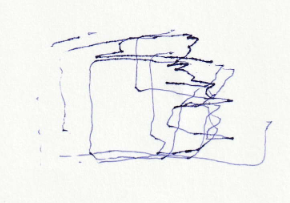
\includegraphics[width=0.90\textwidth]{./img/005.png}
            \caption{生成結果}
            \label{the position of a region}
        \end{figure}
    \end{center}


